\documentclass{extbook}[14pt]
\usepackage{multicol, enumerate, enumitem, hyperref, color, soul, setspace, parskip, fancyhdr, amssymb, amsthm, amsmath, bbm, latexsym, units, mathtools}
\everymath{\displaystyle}
\usepackage[headsep=0.5cm,headheight=0cm, left=1 in,right= 1 in,top= 1 in,bottom= 1 in]{geometry}
\usepackage{dashrule}  % Package to use the command below to create lines between items
\newcommand{\litem}[1]{\item #1

\rule{\textwidth}{0.4pt}}
\pagestyle{fancy}
\lhead{}
\chead{Answer Key for Progress Quiz 10 Version A}
\rhead{}
\lfoot{6232-9639}
\cfoot{}
\rfoot{Fall 2020}
\begin{document}
\textbf{This key should allow you to understand why you choose the option you did (beyond just getting a question right or wrong). \href{https://xronos.clas.ufl.edu/mac1105spring2020/courseDescriptionAndMisc/Exams/LearningFromResults}{More instructions on how to use this key can be found here}.}

\textbf{If you have a suggestion to make the keys better, \href{https://forms.gle/CZkbZmPbC9XALEE88}{please fill out the short survey here}.}

\textit{Note: This key is auto-generated and may contain issues and/or errors. The keys are reviewed after each exam to ensure grading is done accurately. If there are issues (like duplicate options), they are noted in the offline gradebook. The keys are a work-in-progress to give students as many resources to improve as possible.}

\rule{\textwidth}{0.4pt}

\begin{enumerate}\litem{
Determine the domain of the function below.
\[ f(x) = \frac{3}{36x^{2} +12 x -15} \]

The solution is \( \text{All Real numbers except } x = -0.833 \text{ and } x = 0.500. \), which is option E.\begin{enumerate}[label=\Alph*.]
\item \( \text{All Real numbers except } x = a, \text{ where } a \in [-30.2, -27.8] \)

All Real numbers except $x = -30.000$, which corresponds to removing a distractor value from the denominator.
\item \( \text{All Real numbers.} \)

This corresponds to thinking the denominator has complex roots or that rational functions have a domain of all Real numbers.
\item \( \text{All Real numbers except } x = a \text{ and } x = b, \text{ where } a \in [-30.2, -27.8] \text{ and } b \in [17.9, 19.9] \)

All Real numbers except $x = -30.000$ and $x = 18.000$, which corresponds to not factoring the denominator correctly.
\item \( \text{All Real numbers except } x = a, \text{ where } a \in [-2.8, -0.6] \)

All Real numbers except $x = -0.833$, which corresponds to removing only 1 value from the denominator.
\item \( \text{All Real numbers except } x = a \text{ and } x = b, \text{ where } a \in [-2.8, -0.6] \text{ and } b \in [-0.5, 1.6] \)

All Real numbers except $x = -0.833$ and $x = 0.500$, which is the correct option.
\end{enumerate}

\textbf{General Comment:} Recall that dividing by zero is not a real number. Therefore the domain is all real numbers \textbf{except} those that make the denominator 0.
}
\litem{
Choose the equation of the function graphed below.

\begin{center}
    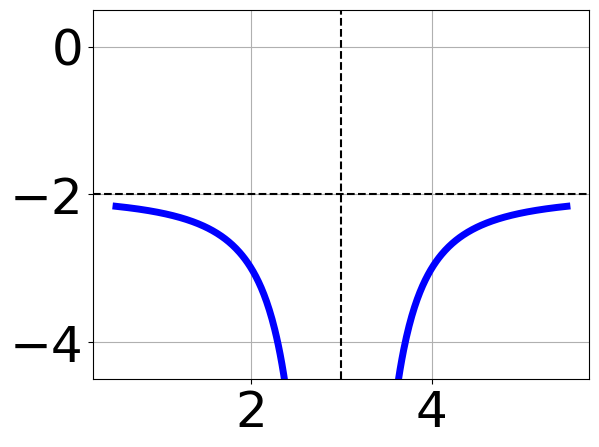
\includegraphics[width=0.5\textwidth]{../Figures/rationalGraphToEquationA.png}
\end{center}




The solution is \( f(x) = \frac{-1}{(x - 3)^2} - 2 \), which is option B.\begin{enumerate}[label=\Alph*.]
\item \( f(x) = \frac{-1}{x - 3} - 2 \)

Corresponds to thinking the graph was a shifted version of $\frac{1}{x}$.
\item \( f(x) = \frac{-1}{(x - 3)^2} - 2 \)

This is the correct option.
\item \( f(x) = \frac{1}{x + 3} - 2 \)

Corresponds to thinking the graph was a shifted version of $\frac{1}{x}$, using the general form $f(x) = \frac{a}{(x+h)^2}+k$, and the opposite leading coefficient.
\item \( f(x) = \frac{1}{(x + 3)^2} - 2 \)

Corresponds to using the general form $f(x) = \frac{a}{(x+h)^2}+k$ and the opposite leading coefficient.
\item \( \text{None of the above} \)

This corresponds to believing the vertex of the graph was not correct.
\end{enumerate}

\textbf{General Comment:} Remember that the general form of a basic rational equation is $ f(x) = \frac{a}{(x-h)^n} + k$, where $a$ is the leading coefficient (and in this case, we assume is either $1$ or $-1$), $n$ is the degree (in this case, either $1$ or $2$), and $(h, k)$ is the intersection of the asymptotes.
}
\litem{
Solve the rational equation below. Then, choose the interval(s) that the solution(s) belongs to.
\[ \frac{6x}{6x + 4} + \frac{-4x^{2}}{42x^{2} +40 x + 8} = \frac{7}{7x + 2} \]

The solution is \( \text{There are two solutions: } x = -0.550 \text{ and } x = 1.340 \), which is option A.\begin{enumerate}[label=\Alph*.]
\item \( x_1 \in [-0.99, -0.54] \text{ and } x_2 \in [1.34,5.34] \)

* $x = -0.550 \text{ and } x = 1.340$, which is the correct option.
\item \( x \in [0.95,1.53] \)


\item \( x_1 \in [-0.99, -0.54] \text{ and } x_2 \in [-5.67,0.33] \)


\item \( \text{All solutions lead to invalid or complex values in the equation.} \)


\item \( x \in [-0.3,0.15] \)


\end{enumerate}

\textbf{General Comment:} Distractors are different based on the number of solutions. Remember that after solving, we need to make sure our solution does not make the original equation divide by zero!
}
\litem{
Solve the rational equation below. Then, choose the interval(s) that the solution(s) belongs to.
\[ \frac{3}{-4x + 8} + 3 = \frac{6}{32x -64} \]

The solution is \( x = 2.312 \), which is option E.\begin{enumerate}[label=\Alph*.]
\item \( x \in [-2.06,-1.42] \)

$x = -1.688$, which corresponds to not distributing the factor $-4x + 8$ correctly when trying to eliminate the fraction.
\item \( x_1 \in [-2.06, -1.42] \text{ and } x_2 \in [0.31,3.31] \)

$x = -1.688 \text{ and } x = 2.312$, which corresponds to getting the correct solution and believing there should be a second solution to the equation.
\item \( x_1 \in [1.28, 2.15] \text{ and } x_2 \in [0.31,3.31] \)

$x = 1.750 \text{ and } x = 2.312$, which corresponds to getting the correct solution and believing there should be a second solution to the equation.
\item \( \text{All solutions lead to invalid or complex values in the equation.} \)

This corresponds to thinking $x = 2.312$ leads to dividing by zero in the original equation, which it does not.
\item \( x \in [1.31,4.31] \)

* $x = 2.312$, which is the correct option.
\end{enumerate}

\textbf{General Comment:} Distractors are different based on the number of solutions. Remember that after solving, we need to make sure our solution does not make the original equation divide by zero!
}
\litem{
Choose the graph of the equation below.
\[ f(x) = \frac{-1}{x - 2} - 2 \]

The solution is the graph below, which is option D.
\begin{center}
    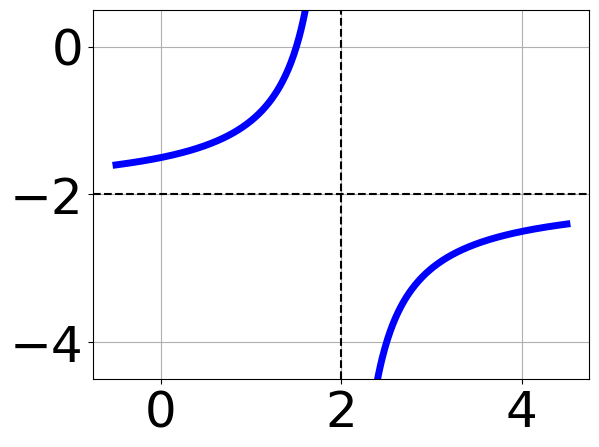
\includegraphics[width=0.3\textwidth]{../Figures/rationalEquationToGraphDA.png}
\end{center}\begin{enumerate}[label=\Alph*.]
\begin{multicols}{2}
\item 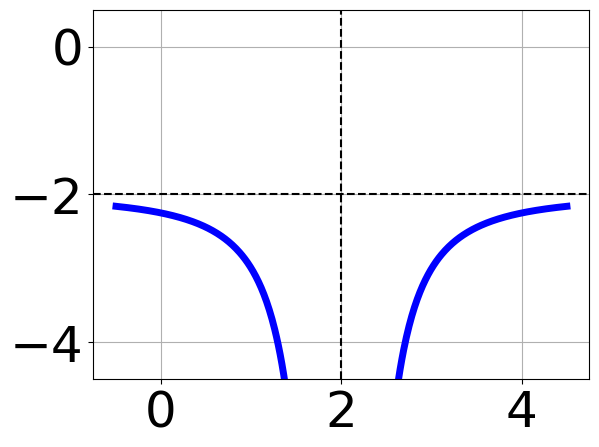
\includegraphics[width = 0.3\textwidth]{../Figures/rationalEquationToGraphAA.png}
\item 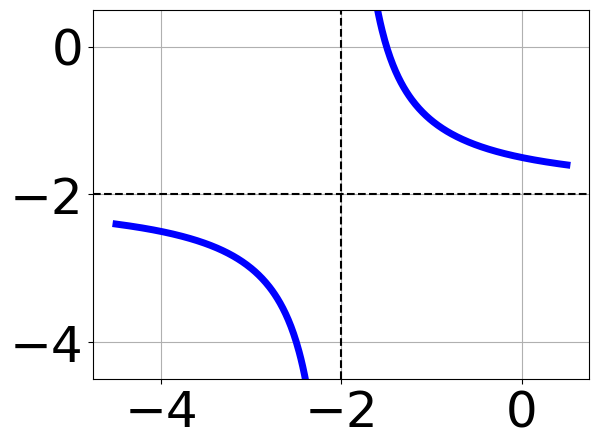
\includegraphics[width = 0.3\textwidth]{../Figures/rationalEquationToGraphBA.png}
\item 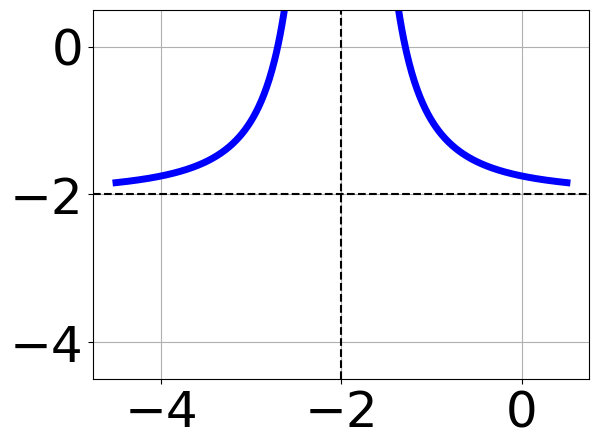
\includegraphics[width = 0.3\textwidth]{../Figures/rationalEquationToGraphCA.png}
\item 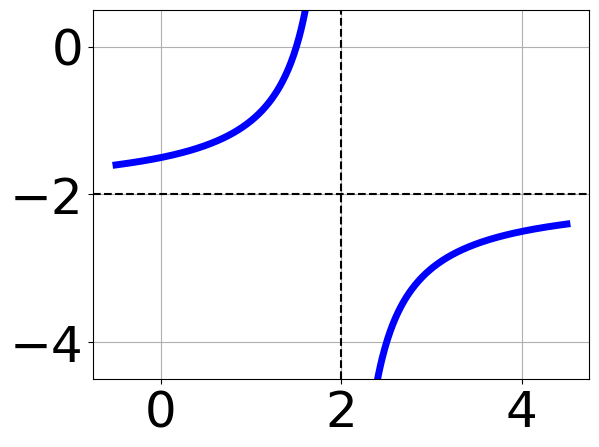
\includegraphics[width = 0.3\textwidth]{../Figures/rationalEquationToGraphDA.png}
\end{multicols}\item None of the above.\end{enumerate}
\textbf{General Comment:} Remember that the general form of a basic rational equation is $ f(x) = \frac{a}{(x-h)^n} + k$, where $a$ is the leading coefficient (and in this case, we assume is either $1$ or $-1$), $n$ is the degree (in this case, either $1$ or $2$), and $(h, k)$ is the intersection of the asymptotes.
}
\litem{
Solve the rational equation below. Then, choose the interval(s) that the solution(s) belongs to.
\[ \frac{-84}{60x + 60} + 1 = \frac{-84}{60x + 60} \]

The solution is \( \text{all solutions are invalid or lead to complex values in the equation.} \), which is option B.\begin{enumerate}[label=\Alph*.]
\item \( x_1 \in [-1.6, -0.7] \text{ and } x_2 \in [-1.1,0.3] \)

$x = -1.000 \text{ and } x = -1.000$, which corresponds to getting the correct solution and believing there should be a second solution to the equation.
\item \( \text{All solutions lead to invalid or complex values in the equation.} \)

*$x = -1.000$ leads to dividing by 0 in the original equation and thus is not a valid solution, which is the correct option.
\item \( x_1 \in [-1.6, -0.7] \text{ and } x_2 \in [-0.3,1.4] \)

$x = -1.000 \text{ and } x = 1.000$, which corresponds to getting the correct solution and believing there should be a second solution to the equation.
\item \( x \in [-1.0,1.0] \)

$x = -1.000$, which corresponds to not checking if this value leads to dividing by 0 in the original equation and thus is not a valid solution.
\item \( x \in [0.4,1.9] \)

$x = 1.000$, which corresponds to not distributing the factor $60x + 60$ correctly when trying to eliminate the fraction.
\end{enumerate}

\textbf{General Comment:} Distractors are different based on the number of solutions. Remember that after solving, we need to make sure our solution does not make the original equation divide by zero!
}
\litem{
Determine the domain of the function below.
\[ f(x) = \frac{3}{18x^{2} -24 x -24} \]

The solution is \( \text{All Real numbers except } x = -0.667 \text{ and } x = 2.000. \), which is option E.\begin{enumerate}[label=\Alph*.]
\item \( \text{All Real numbers except } x = a, \text{ where } a \in [-25, -22] \)

All Real numbers except $x = -24.000$, which corresponds to removing a distractor value from the denominator.
\item \( \text{All Real numbers except } x = a, \text{ where } a \in [-0.67, 0.33] \)

All Real numbers except $x = -0.667$, which corresponds to removing only 1 value from the denominator.
\item \( \text{All Real numbers except } x = a \text{ and } x = b, \text{ where } a \in [-25, -22] \text{ and } b \in [18, 19] \)

All Real numbers except $x = -24.000$ and $x = 18.000$, which corresponds to not factoring the denominator correctly.
\item \( \text{All Real numbers.} \)

This corresponds to thinking the denominator has complex roots or that rational functions have a domain of all Real numbers.
\item \( \text{All Real numbers except } x = a \text{ and } x = b, \text{ where } a \in [-0.67, 0.33] \text{ and } b \in [1, 5] \)

All Real numbers except $x = -0.667$ and $x = 2.000$, which is the correct option.
\end{enumerate}

\textbf{General Comment:} Recall that dividing by zero is not a real number. Therefore the domain is all real numbers \textbf{except} those that make the denominator 0.
}
\litem{
Choose the graph of the equation below.
\[ f(x) = \frac{-1}{x - 2} + 2 \]

The solution is the graph below, which is option E.
\begin{center}
    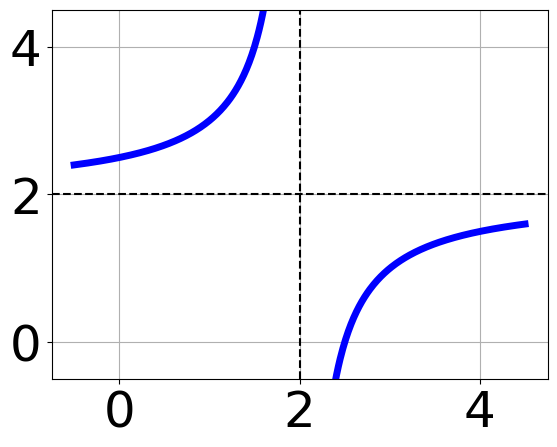
\includegraphics[width=0.3\textwidth]{../Figures/rationalEquationToGraphCopyEA.png}
\end{center}\begin{enumerate}[label=\Alph*.]
\begin{multicols}{2}
\item 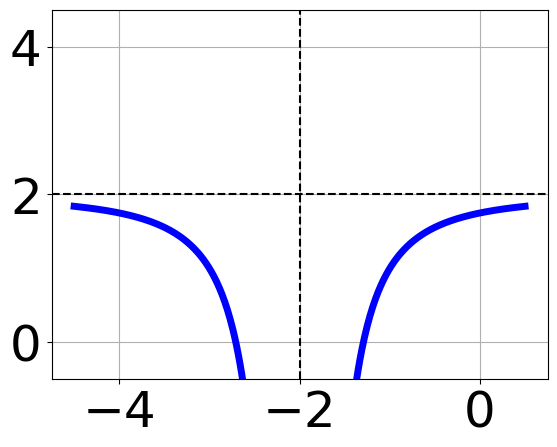
\includegraphics[width = 0.3\textwidth]{../Figures/rationalEquationToGraphCopyAA.png}
\item 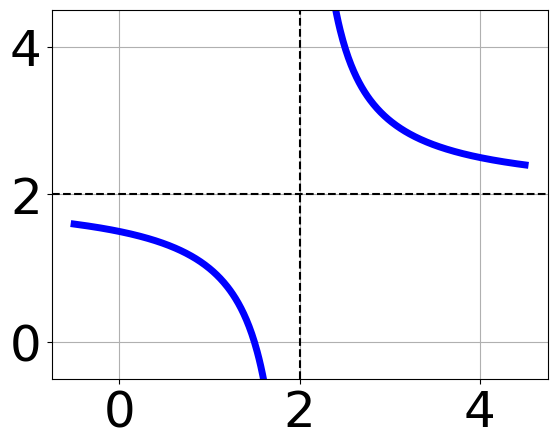
\includegraphics[width = 0.3\textwidth]{../Figures/rationalEquationToGraphCopyBA.png}
\item 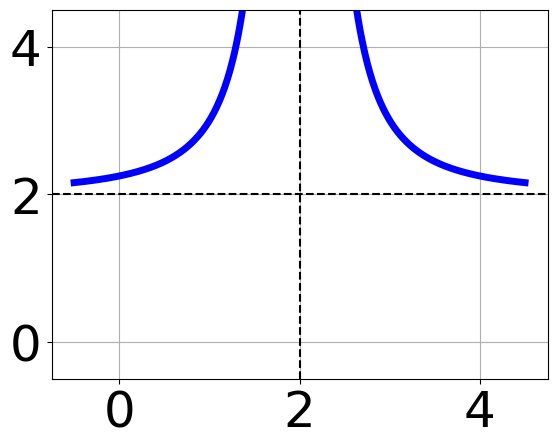
\includegraphics[width = 0.3\textwidth]{../Figures/rationalEquationToGraphCopyCA.png}
\item 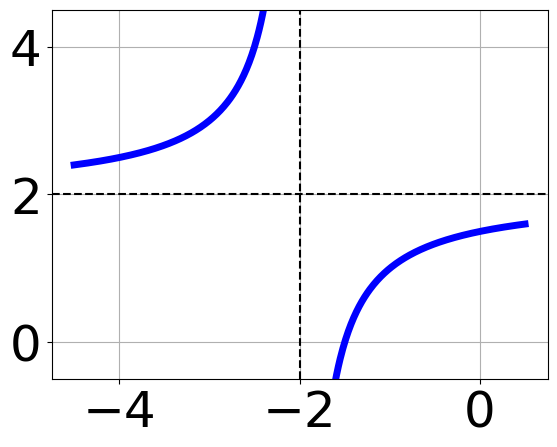
\includegraphics[width = 0.3\textwidth]{../Figures/rationalEquationToGraphCopyDA.png}
\end{multicols}\item None of the above.\end{enumerate}
\textbf{General Comment:} Remember that the general form of a basic rational equation is $ f(x) = \frac{a}{(x-h)^n} + k$, where $a$ is the leading coefficient (and in this case, we assume is either $1$ or $-1$), $n$ is the degree (in this case, either $1$ or $2$), and $(h, k)$ is the intersection of the asymptotes.
}
\litem{
Choose the equation of the function graphed below.

\begin{center}
    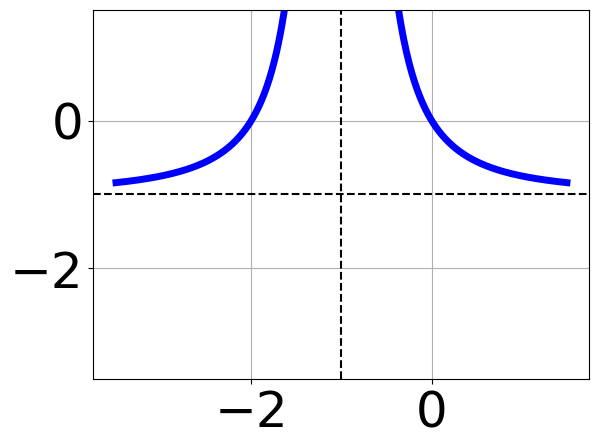
\includegraphics[width=0.5\textwidth]{../Figures/rationalGraphToEquationCopyA.png}
\end{center}




The solution is \( f(x) = \frac{1}{(x + 1)^2} - 1 \), which is option A.\begin{enumerate}[label=\Alph*.]
\item \( f(x) = \frac{1}{(x + 1)^2} - 1 \)

This is the correct option.
\item \( f(x) = \frac{-1}{(x - 1)^2} - 1 \)

Corresponds to using the general form $f(x) = \frac{a}{(x+h)^2}+k$ and the opposite leading coefficient.
\item \( f(x) = \frac{1}{x + 1} - 1 \)

Corresponds to thinking the graph was a shifted version of $\frac{1}{x}$.
\item \( f(x) = \frac{-1}{x - 1} - 1 \)

Corresponds to thinking the graph was a shifted version of $\frac{1}{x}$, using the general form $f(x) = \frac{a}{(x+h)^2}+k$, and the opposite leading coefficient.
\item \( \text{None of the above} \)

This corresponds to believing the vertex of the graph was not correct.
\end{enumerate}

\textbf{General Comment:} Remember that the general form of a basic rational equation is $ f(x) = \frac{a}{(x-h)^n} + k$, where $a$ is the leading coefficient (and in this case, we assume is either $1$ or $-1$), $n$ is the degree (in this case, either $1$ or $2$), and $(h, k)$ is the intersection of the asymptotes.
}
\litem{
Solve the rational equation below. Then, choose the interval(s) that the solution(s) belongs to.
\[ \frac{-6x}{-5x -4} + \frac{-4x^{2}}{15x^{2} -23 x -28} = \frac{-4}{-3x + 7} \]

The solution is \( \text{There are two solutions: } x = -0.245 \text{ and } x = 4.673 \), which is option B.\begin{enumerate}[label=\Alph*.]
\item \( x_1 \in [-1.22, 1.87] \text{ and } x_2 \in [-0.8,0.2] \)


\item \( x_1 \in [-1.22, 1.87] \text{ and } x_2 \in [4.67,6.67] \)

* $x = -0.245 \text{ and } x = 4.673$, which is the correct option.
\item \( x \in [1.37,4.17] \)


\item \( \text{All solutions lead to invalid or complex values in the equation.} \)


\item \( x \in [3.16,6.6] \)


\end{enumerate}

\textbf{General Comment:} Distractors are different based on the number of solutions. Remember that after solving, we need to make sure our solution does not make the original equation divide by zero!
}
\end{enumerate}

\end{document}